
\stagedivider{5}{Epilogue: Trust}{What do you trust, and why?}

\begin{frame}{Currently, Claude is approved for public data only at ND}
  \vfill
  \renewcommand{\arraystretch}{0.9}
  \begin{center}
  \begin{tabular}{@{}lll@{}}
    \toprule
    \textbf{Tier} & \textbf{Examples} & \textbf{AI use} \\
    \midrule
    \textcolor{OkGreen}{$\bullet$}~Public    & published, press-released & safe \\
    \textcolor{NDGold!80!black}{$\bullet$}~Internal  & routine business data & safe \emph{in approved tools} \\
    \textcolor{OkVermillion}{$\bullet$}~Sensitive & role-restricted       & safe \emph{in approved tools} \\
    \textcolor{black}{$\blacksquare$}~Restricted & SSN, health, payment  & \bad{never, in any tool} \\
    \bottomrule
  \end{tabular}
  \end{center}
  \vspace{0.5em}
  \begin{center}
  \begin{tabular}{@{}lc@{}}
    \toprule
    \textbf{Tool} & \textbf{Approved through} \\
    \midrule
    Gemini, ChatGPT EDU, NotebookLM & Sensitive \\
    \textbf{Claude} & \textbf{Public only} \\
    \bottomrule
  \end{tabular}
  \end{center}
  \renewcommand{\arraystretch}{1}
  \vspace{0.5em}
  \begin{center}
    \small Claude Team accounts (free for academic labs) do not train on your data by default, but have a risk/reward conversation with your PI.
  \end{center}
  \vspace{1.8cm plus 1fill}
\end{frame}

\begin{frame}{Two important notes}
  \vfill
  \begin{itemize}\setlength\itemsep{1.2em}
    \item \textbf{DoD / DoW funding?}\\
      Certain funding agencies currently \bad{prohibit}
      using any Anthropic product --- Claude.ai, the API, Claude
      Code.\\[0.3em]
      {\small Questions: \texttt{researchsecurity@nd.edu} (CC your PI)}
    \item \textbf{Everyone else: ask your PI.}\\
      Export control, sponsor terms, intellectual property protection, and IRB conditions differ per
      project
  \end{itemize}
  \vfill
\end{frame}

\begin{frame}{The same tasks recur across projects and acts}
  \vfill
  \begin{center}
  \small
  \begin{tabular}{@{}lccccc@{}}
    \toprule
    & \textbf{Prologue} & \textbf{Act I} & \textbf{Act II} & \textbf{Act III} \\
    \midrule
    Task 1 --- set up git & & \good{} & & \\
    Task 2 --- inherit a project's context & & \good{} & & \\
    Task 3 --- idea $\to$ report or proposal & & \good{} & \good{} & \\
    Task 4 --- paper code $\to$ package & \good{} & & \good{} & \\
    Task 5 --- audit a manuscript & & & & \good{} \\
    Task 6 --- inherit a project $\to$ manuscript & & & & \good{} \\
    Task 7 --- audit a course, end to end & & & & \good{} \\
    Creating this talk & \good{} & & & \\
    \bottomrule
  \end{tabular}
  \end{center}
  \vfill
  \begin{center}
    Tasks 1--7 form the research workflow. Task 8 is the hobby extension.
  \end{center}
  \vfill
\end{frame}

\begin{frame}{You own every claim, whatever helped you make it}
  \vfill
  \begin{itemize}\setlength\itemsep{0.9em}
    \item AI drafts, checks, and challenges. It does not decide what's true.
    \item Disclose AI use the way you'd disclose a collaborator's contribution --- journals increasingly expect it named as a research method, not left in a footnote.
    \item I checked factual claims against primary evidence before they went on a slide. Personal estimates remain labeled as such.
    \item The same standard applies to your own work, whatever helped you produce it.
  \end{itemize}
  \vfill
\end{frame}

\begin{frame}{Task 8 (hobbies) --- using AI to amplify your curiosity}
  \vfill
  \begin{columns}[c]
    \begin{column}{0.48\textwidth}
      \centering
      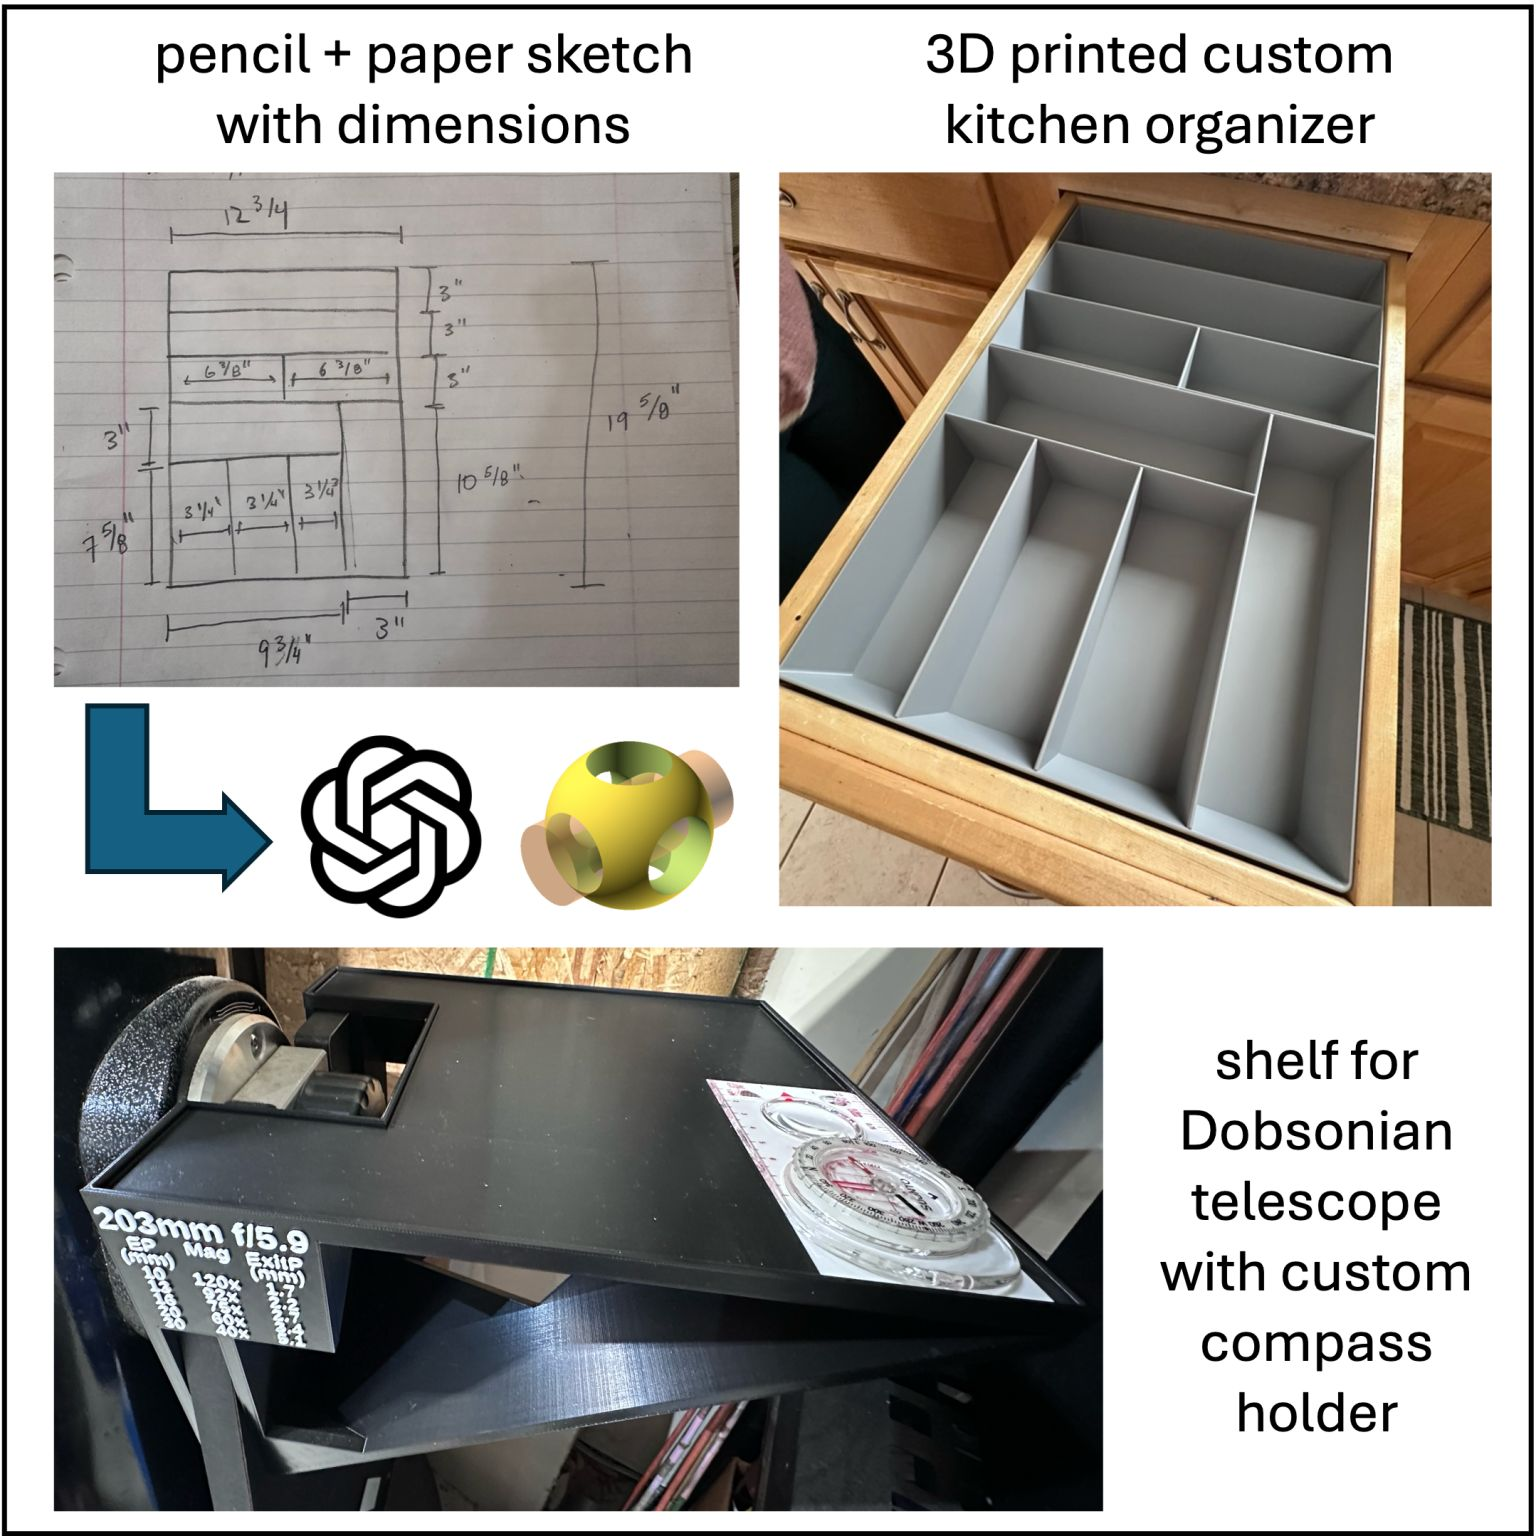
\includegraphics[height=5.2cm]{figures/kitchen_organizer_telescope_shelf.jpeg}
    \end{column}
    \begin{column}{0.46\textwidth}
      \textbf{\small My workflow}
      \begin{enumerate}\small\setlength\itemsep{0.05em}
        \item Sketch on paper, or lately, photos with a tape measure/caliper
        \item \texttt{init\_project.sh}; design in OpenSCAD, iterating with Codex against \texttt{STYLE.md}
        \item \texttt{render\_views.sh} for views --- falls back to Blender on OpenSCAD crashes
        \item Look at the views, tell Codex what's wrong, repeat until it matches the sketch
      \end{enumerate}
      \vspace{0.1em}
      \textbf{\small Projects}
      \begin{itemize}\small\setlength\itemsep{0.05em}
        \item boot dryer, bathroom \& drawer organizers, telescope shelf \& caps
        \item camera \& binocular mounts, CBE keychains (recruitment), tablet car mount (kids)
      \end{itemize}
    \end{column}
  \end{columns}
  \vspace{0.1cm plus 1fill}
\end{frame}

\begin{frame}{Task 8 (hobbies) --- create a textbook, customized for you}
  \ndlogonote{\scriptsize\href{https://github.com/adowling2/radio-extra-book}{\texttt{github.com/adowling2/radio-extra-book}}}
  \vfill
  \begin{center}
    I want to \textbf{learn} AC circuit theory rather than memorize answers for the top-level \textbf{amateur radio license exam}. With Claude, I created a \textbf{personalized textbook}.
  \end{center}
  \vspace{0.35em}
  \begin{columns}[c]
    \begin{column}{0.40\textwidth}
      \textbf{\small My approach}
      \begin{enumerate}\small\setlength\itemsep{0.1em}
        \item Brainstorm with ChatGPT the connections between AC circuit theory and my background
        \item Draft the source, chapter by chapter
        \item Reorganize into a coherent part structure
        \item Build a reproducible figure pipeline
        \item Verify coverage against real exam question pools
        \item Revise in structured rounds
      \end{enumerate}
    \end{column}
    \begin{column}{0.56\textwidth}
      \centering
      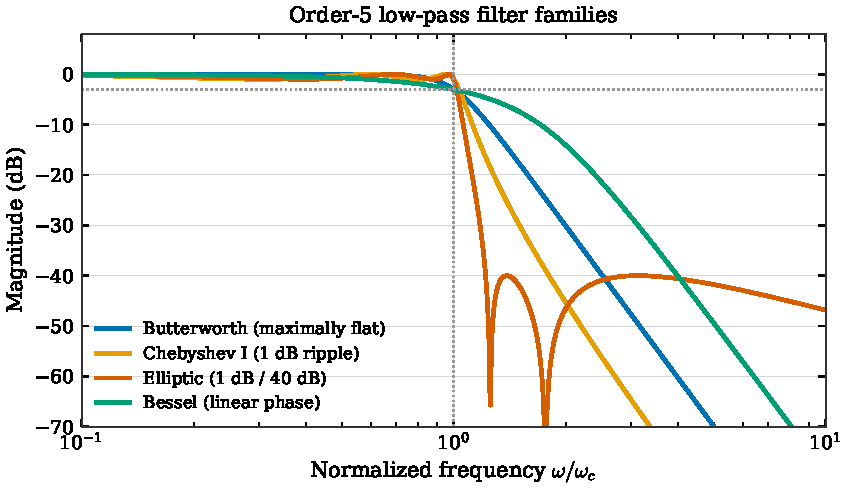
\includegraphics[width=0.8\linewidth]{figures/filter_families}\\[0.05em]
      {\scriptsize I want to understand the math behind filters on the Amerature Extra exam.}
    \end{column}
  \end{columns}
  \vspace{0.6cm plus 1fill}
\end{frame}

\begin{frame}[fragile]{So, what now?}
  \vfill
  \begin{center}
  \begin{enumerate}\normalsize\setlength\itemsep{0.35em}
    \item Create a \textbf{GitHub} account (use your \texttt{.edu} email and apply for a free Education, a.k.a., Pro, upgrade)
    \item Install \textbf{GitHub Desktop}: \url{https://desktop.github.com/download/}
    \item \textbf{Clone this repo}: \texttt{github.com/dowlinglab/claude-for-researchers}
    \item Open an \textbf{AI agent} in the repo: Codex, Claude Code, Gemini CLI, etc.
    \item Paste in the starter prompt from \href{https://github.com/dowlinglab/claude-for-researchers/blob/main/resources/prompts/getting_started.md}{\texttt{resources/prompts/getting\_started.md}}
    \item \textbf{Have a real conversation}: your project, your pain points, ask for help
  \end{enumerate}
  \end{center}
  \vspace{0.6em}
  \begin{center}
    \slidepoint{The resources in this repo provide a starting place. But remember, anything in this talk could become outdate/stale tomorrow.}
  \end{center}
  \vfill
\end{frame}
